% =============================================================================
% Soutenance finale — 20 minutes
% Fil rouge : bloc opératoire, lits d'hospitalisation et ambulatoire.
%
% Découpage : Contextualiser (3) — Problématique (2) — Modélisation (8)
%             — Résultats (3) — Application (7)
%
% Compilation depuis soutenance/final/ :
%   lualatex Soutenance_finale.tex
%   biber    Soutenance_finale
%   lualatex Soutenance_finale.tex
%   lualatex Soutenance_finale.tex
% =============================================================================
\documentclass[aspectratio=169,11pt]{beamer}
\usepackage{../beamerthememidcenturymodern}
\mcmTheme{Kraft}

\definecolor{McmTerracotta}{HTML}{9C4732}
\definecolor{McmSage}{HTML}{6B7F3A}
\definecolor{McmAmber}{HTML}{DB6720}
\definecolor{McmWarm}{HTML}{F8F6F2}
\definecolor{McmSand}{HTML}{E8D5B5}
\definecolor{McmInk}{HTML}{1A1A1A}
\definecolor{McmMuted}{HTML}{5A534E}

\usepackage[french]{babel}
\usepackage{amsmath,amssymb}
\usepackage{booktabs}
\usepackage{tikz}
\usetikzlibrary{arrows.meta,positioning,calc,babel,backgrounds,fit,shapes.geometric}
\usepackage{graphicx}
\graphicspath{{photos/}{../figures/}}

\newcommand{\source}[1]{\par\vspace{4pt}{\color{mcmBlack!60}\tiny #1}}
\newcommand{\credit}[1]{\par\vspace{2pt}{\color{mcmBlack!55}\tiny #1}}
\newcommand{\bigstat}[2]{%
  \begin{minipage}{\linewidth}\centering
    {\fontsize{23}{25}\selectfont\bfseries\color{mcmPrimary}#1}\par
    \vspace{-1pt}
    {\scriptsize\color{mcmBlack!75}#2}\par
  \end{minipage}}
\newcommand{\partnum}[1]{{\color{mcmPrimary}\bfseries #1}}

\title[Bloc, lits \& ambulatoire]{Optimiser ensemble le bloc, les lits et l'ambulatoire}
\subtitle{Du planning contraint à la décision explicable}
\author[IA \& Santé --- Groupe 2]{IA et Santé --- Groupe 2}
\date{Soutenance finale --- 2026}

\begin{document}

\begin{frame}[plain]
  \titlepage
\end{frame}

\section{Fil rouge}

\begin{frame}{Le fil rouge}
  \footnotesize
      \begin{tabular}{@{}p{2cm}p{11cm}@{}}
        \partnum{1} & \textbf{Contextualiser} \\
        \partnum{2} & \textbf{Problématique} \\
        \partnum{3} & \textbf{Modéliser et approcher} \\
        \partnum{4} & \textbf{Analyser les résultats} \\
        \partnum{5} & \textbf{Montrer l'application} \\
      \end{tabular}
      \uncover<2->{%
      \vspace{0.2cm}
      \begin{alertblock}{Objectif}
        \small Décider plus tôt, avec des dates justifiées, sans décider à la
        place du praticien.
      \end{alertblock}}
\end{frame}

\section{Contextualiser}

\begin{frame}{Le bloc opératoire, une ressource rare et non stockable}
  \small
  \begin{columns}[T,onlytextwidth]
    \begin{column}{0.41\textwidth}
      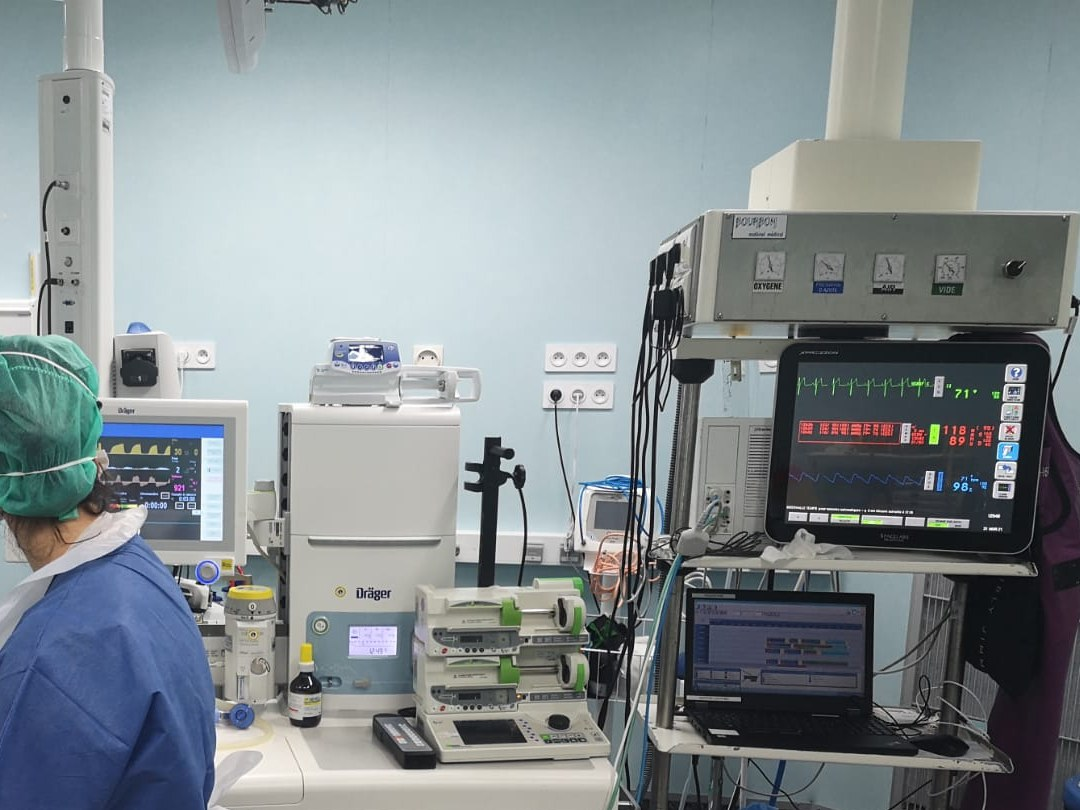
\includegraphics[width=\linewidth]{photo_bloc.jpg}
      \credit{Photo : Hirondus, CC BY-SA 4.0, Wikimedia Commons.}
    \end{column}

    \begin{column}{0.55\textwidth}
      \begin{columns}[T,onlytextwidth]
        \begin{column}{0.32\textwidth}\centering
          \bigstat{64,4\,\%}{taux national d'ambulatoire en 2023}
        \end{column}
        \begin{column}{0.32\textwidth}\centering
          \bigstat{70\,\%}{objectif national fixé pour 2022}
        \end{column}
        \begin{column}{0.32\textwidth}\centering
          \bigstat{80\,\%}{cap affiché pour la suite}
        \end{column}
      \end{columns}

      \uncover<2->{%
      \vspace{0.18cm}
      \begin{block}{Enjeux}
        \footnotesize
        Une salle, une équipe et un lit mobilisés sans patient coûtent sans
        soigner. L'objectif national et l'autorisation ARS rendent la décision
        traçable ; l'ambulatoire réduit le risque infectieux et accélère
        l'accès.
      \end{block}}
    \end{column}
  \end{columns}
  \source{Sources : HAS, IQSS (avril 2026) ; HAS, 12 questions (2012).}
\end{frame}

\begin{frame}{Du flux poussé au flux tiré}
  \scriptsize
  \begin{columns}[T,onlytextwidth]
    \begin{column}{0.58\textwidth}
      \only<1>{%
      \begin{block}{Aujourd'hui : flux poussé}
        \centering
        \begin{tikzpicture}[
          b/.style={draw=McmTerracotta,rounded corners=2pt,fill=white,
                    text width=1.85cm,minimum height=1.0cm,align=center,
                    font=\scriptsize,inner sep=2pt},
          f/.style={-{Latex[length=2mm]},thick,draw=McmTerracotta}]
          \node[b] (a) at (0,0) {Le chirurgien\\choisit une date};
          \node[b] (b) at (3.0,0) {Bloc, lits et\\équipes s'adaptent};
          \node[b] (c) at (6.0,0) {Pics et creux\\d'activité};
          \draw[f] (a) -- (b);
          \draw[f] (b) -- (c);
        \end{tikzpicture}
      \end{block}}

      \only<2->{%
      \begin{exampleblock}{Demain : flux tiré}
        \centering
        \begin{tikzpicture}[
          b/.style={draw=McmSage,rounded corners=2pt,fill=white,
                    text width=1.85cm,minimum height=1.0cm,align=center,
                    font=\scriptsize,inner sep=2pt},
          f/.style={-{Latex[length=2mm]},thick,draw=McmSage}]
          \node[b] (a) at (0,0) {Ressources et\\contraintes};
          \node[b] (b) at (3.0,0) {Dates A et B\\calculées};
          \node[b] (c) at (6.0,0) {Le chirurgien\\choisit};
          \draw[f] (a) -- (b);
          \draw[f] (b) -- (c);
        \end{tikzpicture}
      \end{exampleblock}}

      \uncover<3->{\par\vspace{0.15cm}\centering\footnotesize
        Le planning propose des dates compatibles ; le praticien arbitre.}
    \end{column}

    \begin{column}{0.40\textwidth}
      \centering
      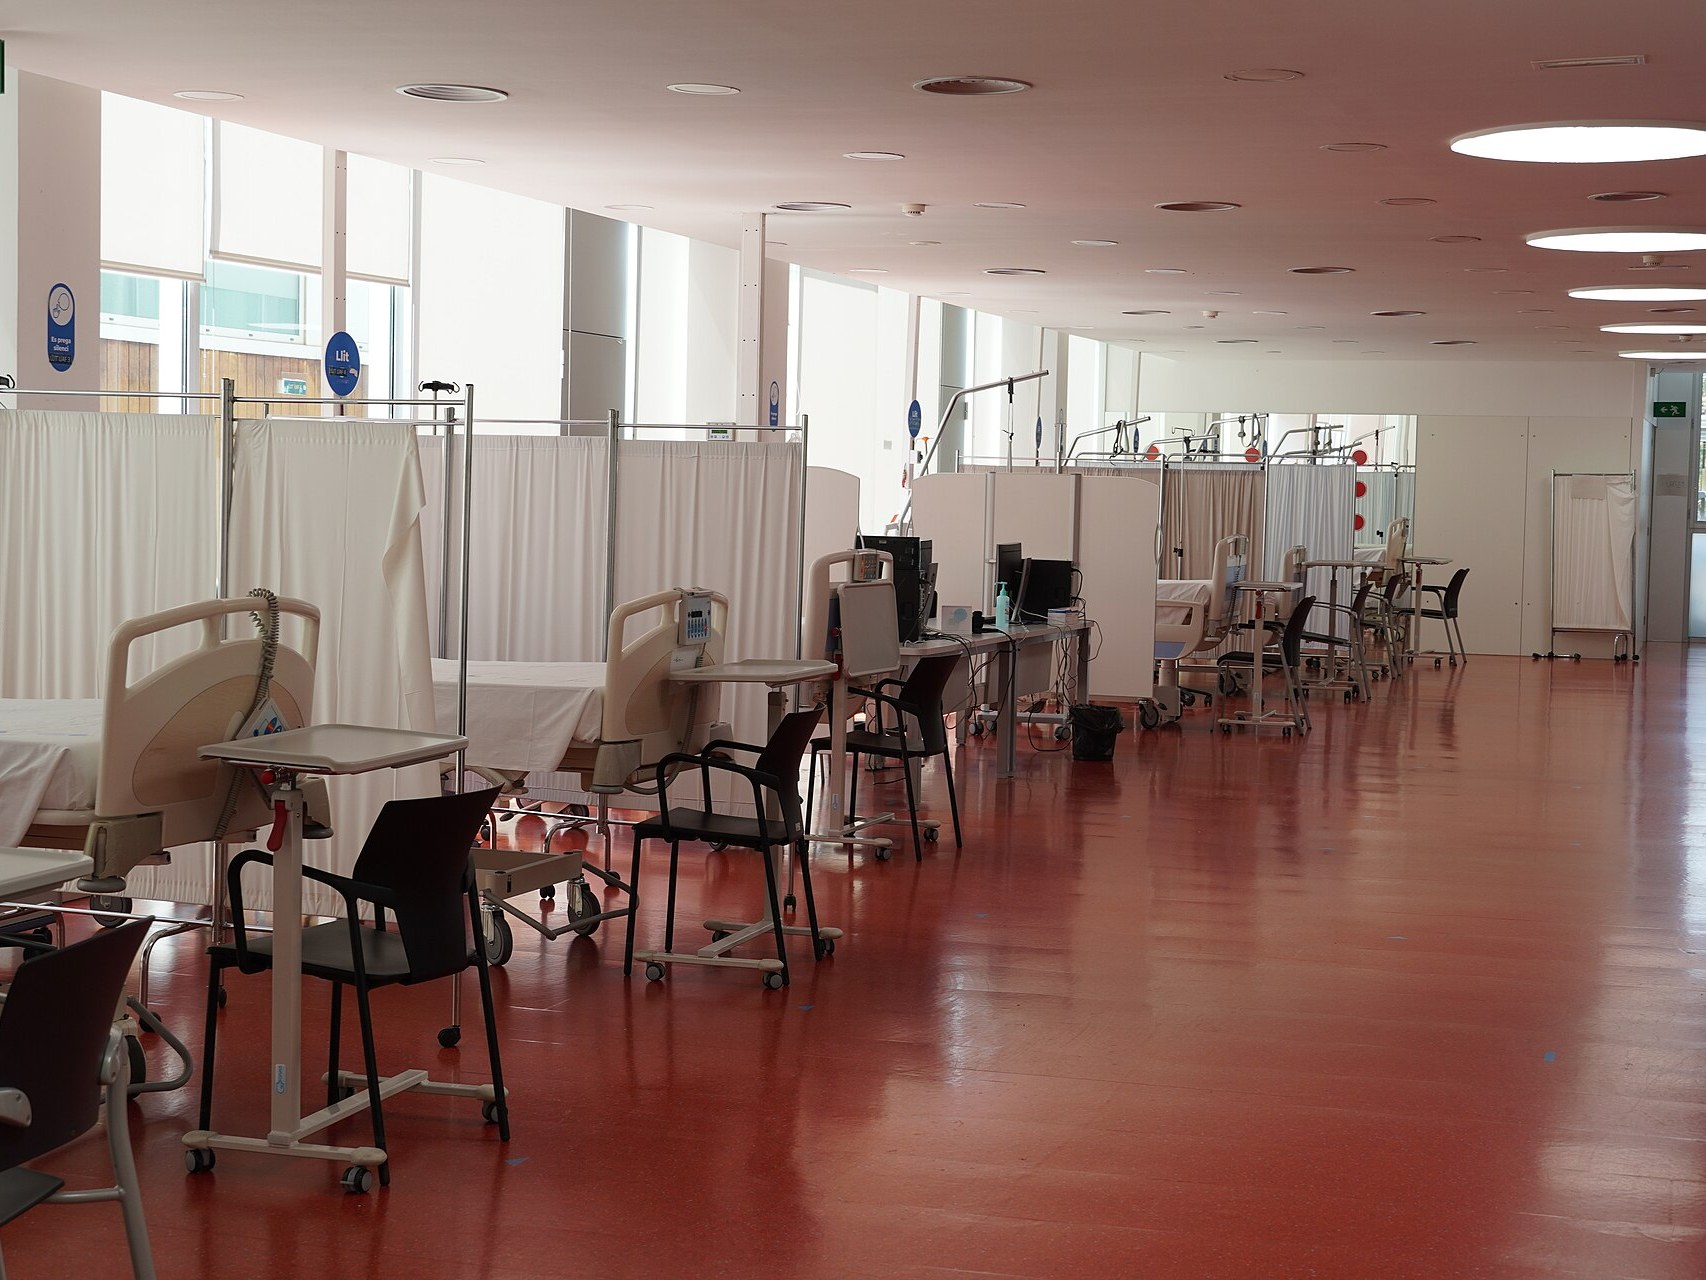
\includegraphics[width=0.88\linewidth]{photo_lits.jpg}
      \credit{Photo : Ncsi24, CC BY-SA 4.0, Wikimedia Commons.}
      \par\vspace{0.12cm}
      {\footnotesize Un séjour de plusieurs jours engage la capacité de
        demain.}
    \end{column}
  \end{columns}
\end{frame}

\begin{frame}{Ce que fait l'application, et ce qu'elle ne fait pas}
  \small
  \begin{columns}[T,onlytextwidth]
    \begin{column}{0.56\textwidth}
      \begin{enumerate}
        \item<1-> Le chirurgien saisit la demande en consultation.
        \item<1-> Le moteur prédit les durées et l'hébergement.
        \item<2-> L'outil propose \textbf{deux dates}, avec leurs raisons.
        \item<2-> Le chirurgien confirme : vacation et lit sont réservés.
      \end{enumerate}

      \uncover<3->{\par\vspace{0.15cm}\footnotesize
        L'outil ne programme pas à la place du praticien. Il rend les
        conséquences d'un choix visibles avant la confirmation.}
    \end{column}

    \begin{column}{0.42\textwidth}
      \centering
      \begin{tikzpicture}[font=\scriptsize]
        \draw[rounded corners=9pt,fill=white,draw=McmTerracotta,thick]
          (0,0) rectangle (4.15,6.05);
        \draw[fill=McmTerracotta!10,rounded corners=4pt]
          (0.18,5.35) rectangle (3.97,5.90);
        \node[font=\footnotesize\bfseries,text=McmTerracotta] at (2.08,5.62)
          {Demande};
        \node[align=left,anchor=west] at (0.28,4.95)
          {\textbf{Mme D., 58 ans}\\Chirurgie digestive};
        \draw[draw=McmMuted!35] (0.25,4.55) -- (3.90,4.55);
        \node[align=left,anchor=west] at (0.28,4.25)
          {Durée prédite : \textbf{95 min}\\Séjour : \textbf{2 jours}};
        \draw[fill=McmSage!12,rounded corners=3pt]
          (0.25,2.75) rectangle (3.90,3.95);
        \node[align=left,anchor=west] at (0.35,3.55)
          {\textbf{Date A} --- 12 mars\\{\color{McmSage}bloc et lit disponibles}};
        \draw[fill=McmAmber!12,rounded corners=3pt]
          (0.25,1.45) rectangle (3.90,2.60);
        \node[align=left,anchor=west] at (0.35,2.25)
          {\textbf{Date B} --- 26 mars\\{\color{McmAmber}lits plus tendus le 19}};
        \draw[fill=McmTerracotta,rounded corners=3pt]
          (0.55,0.45) rectangle (3.60,1.05);
        \node[text=white,font=\scriptsize\bfseries] at (2.08,0.75)
          {Confirmer une date};
      \end{tikzpicture}
    \end{column}
  \end{columns}
  \source{Maquette de l'écran de décision. Le parcours complet est en
    partie 5.}
\end{frame}

\section{Problématique}

\begin{frame}{Du terrain au problème}
  \footnotesize
  \begin{columns}[T,onlytextwidth]
    \begin{column}{0.50\textwidth}
      \begin{block}{Le terrain}
        \begin{itemize}
          \item 582 patients, 280 vacations sur 40 jours.
          \item Trois ressources couplées : bloc, lits, ambulatoire.
          \item Quatre aléas : urgence, annulation, fermeture, retard.
        \end{itemize}
      \end{block}

      \uncover<2->{%
      \begin{alertblock}{Le nombre d'affectations}
        \[
          \underbrace{280^{582}}_{\text{affectations possibles}}
        \]
        \footnotesize Les compatibilités réduisent l'espace, sans le rendre
        traitable.
      \end{alertblock}}
    \end{column}

    \begin{column}{0.48\textwidth}
      \centering
      \begin{tikzpicture}[
        c/.style={draw=McmTerracotta,rounded corners=3pt,fill=white,
                  text width=4.5cm,minimum height=1.10cm,align=center,
                  font=\footnotesize,inner sep=3pt},
        f/.style={-{Latex[length=2.5mm]},thick,draw=McmTerracotta}]
        \node[c] (a) at (0,0) {\textbf{Terrain}\\3 ressources, 4 aléas};
        \node[c] (b) at (0,-1.7) {\textbf{Modèle}\\affectation sous contraintes};
        \node<2->[c,draw=McmAmber,fill=McmAmber!8] (c) at (0,-3.3)
          {\textbf{Problème NP-difficile}\\qualité en temps borné};
        \draw[f] (a) -- (b);
        \draw<2->[f,draw=McmAmber] (b) -- (c);
      \end{tikzpicture}
      \uncover<3->{\par\vspace{0.15cm}\footnotesize Dix méthodes, un même
        budget de temps.}
    \end{column}
  \end{columns}
  \source{Charges et protocoles : RAPPORT.md.}
\end{frame}

\begin{frame}{Les contraintes du terrain}
  \scriptsize
  \begin{columns}[T,onlytextwidth]
    \begin{column}{0.49\textwidth}
      \begin{block}{À l'exécution}
        \begin{itemize}
          \item \textbf{Gel du passé} : un acte commencé ou programmé avant le
            jour courant n'est jamais déplacé.
          \item \textbf{Urgences} : insertion dans la fenêtre clinique, pas dès
            qu'une place reste.
          \item \textbf{Moindre perturbation} : déplacer le moins possible les
            patients déjà prévenus.
        \end{itemize}
      \end{block}
    \end{column}

    \begin{column}{0.49\textwidth}
      \begin{alertblock}{CE et RGPD}
        \begin{itemize}
          \item \textbf{CE} : logiciel d'aide à la décision à qualifier au
            titre du règlement (UE) 2017/745.
          \item \textbf{RGPD} : minimisation, pseudonymisation, base légale,
            hébergement de données de santé.
          \item \textbf{Audit} : qui a décidé quoi, quand et pourquoi.
        \end{itemize}
      \end{alertblock}
    \end{column}
  \end{columns}

  \uncover<2->{\par\vspace{0.12cm}\footnotesize Le gel, la traçabilité et
    l'explicabilité contraignent le voisinage, le score et l'interface.}
  \source{Sources : règlement (UE) 2017/745 ; RGPD (UE) 2016/679.}
\end{frame}

\section{Modéliser et approcher}

\begin{frame}{Le modèle : affecter chaque patient à une vacation}
  \scriptsize
  \begin{columns}[T,onlytextwidth]
    \begin{column}{0.46\textwidth}
      \begin{block}{Décision}
        \[
          x_{i,v}\in\{0,1\},\qquad
          \sum_{v\in V_i}x_{i,v}=1
        \]
        \begin{tabular}{@{}ll@{}}
          $x_{i,v}$ & patient $i$ affecté à la vacation $v$ \\
          $V_i$ & vacations compatibles \\
          $d_i$ & durée opératoire estimée \\
        \end{tabular}
      \end{block}

      \uncover<2->{%
      \begin{block}{Contraintes dures}
        \begin{itemize}
          \item une vacation par patient ;
          \item capacité de vacation non dépassée ;
          \item capacité de lits respectée chaque jour ;
          \item fenêtre clinique des urgences respectée.
        \end{itemize}
      \end{block}}
    \end{column}

    \begin{column}{0.52\textwidth}
      \begin{alertblock}{Objectif}
        \[
          \min\; \alpha\,\Delta_{\text{vac}}
          +\beta\,\Delta_{\text{lits}}
          +\gamma\,\sigma_{\text{vac}}
        \]
        \[
          \alpha=5{,}0,\qquad \beta=3{,}0,\qquad \gamma=0{,}05
        \]
        \begin{itemize}
          \item $\Delta_{\text{vac}}$ : minutes au-delà des vacations ;
          \item $\Delta_{\text{lits}}$ : dépassement de capacité en lits ;
          \item $\sigma_{\text{vac}}$ : écart-type de charge des vacations.
        \end{itemize}
      \end{alertblock}
    \end{column}
  \end{columns}
\end{frame}

\begin{frame}{Pipeline ML}
  \scriptsize
  \begin{columns}[T,onlytextwidth]
    \begin{column}{0.47\textwidth}
      \centering
      \begin{tikzpicture}[
        n/.style={draw=McmTerracotta,rounded corners=3pt,fill=white,
                  text width=4.1cm,minimum height=0.75cm,align=center,
                  font=\scriptsize,inner sep=2pt},
        f/.style={-{Latex[length=2mm]},thick,draw=McmTerracotta}]
        \node[n] (a) at (0,0) {\textbf{Données brutes}\\14\,434 cas, 30 colonnes};
        \node[n] (b) at (0,-1.15) {\textbf{Nettoyage}\\73 exclusions, séjour corrigé};
        \node[n] (c) at (0,-2.30) {\textbf{Split temporel par patient}\\2019--2021 $\rightarrow$ 2022};
        \node[n] (d) at (0,-3.45) {\textbf{Trois cibles}\\salle, séjour, ambulatoire};
        \draw[f] (a) -- (b);
        \draw[f] (b) -- (c);
        \draw[f] (c) -- (d);
      \end{tikzpicture}
    \end{column}

    \begin{column}{0.51\textwidth}
      \begin{alertblock}{Les pièges traités}
        \begin{itemize}
          \item valeurs manquantes explicites, sans imputation inventée ;
          \item heures nulles exclues, pas imputées ;
          \item aucune fuite : dates, durées et identifiants exclus.
        \end{itemize}
      \end{alertblock}

      \uncover<2->{\par\vspace{0.12cm}\footnotesize \textbf{Sorties :} durée en salle,
        durée de séjour, ambulatoire}
    \end{column}
  \end{columns}
  \source{Notebooks de prétraitement du dépôt.}
\end{frame}

\begin{frame}{Trois métaheuristiques}
  \footnotesize
  NP-difficile : on cherche une bonne solution en temps borné, avec la même
  interface pour toutes les méthodes.

  \vspace{0.15cm}
  \renewcommand{\arraystretch}{1.18}
  \begin{tabular}{p{2.9cm}p{4.5cm}p{4.5cm}}
    \toprule
    \textbf{Méthode} & \textbf{Principe} & \textbf{Effet} \\
    \midrule
    Recuit simulé & Explorer largement, accepter de remonter
      & Évite les optima locaux \\
    Recherche Tabou & Intensifier le meilleur voisin non tabou
      & Mémoire des mouvements, évite le cyclage \\
    Algorithme génétique & Croiser une population de solutions
      & Diversité ; recombine de bonnes parties \\
    \bottomrule
  \end{tabular}

  \uncover<2->{\par\vspace{0.18cm}\footnotesize Les hybrides enchaînent une
    exploration globale et une intensification locale.}
  \source{Formulation du projet ; revues Amin et al. (2024) et Rachuba et
    al. (2024).}
\end{frame}

\begin{frame}{Solution proposé : Hybrides}
  \footnotesize
  \begin{columns}[T,onlytextwidth]
    \begin{column}{0.54\textwidth}
      \begin{block}{Quatre hybrides}
        \begin{itemize}
          \item \textbf{Tabou $\times$ Recuit} : voisinage tabou et acceptation
            de Metropolis.
          \item \textbf{Génétique $\times$ Tabou} : tabou courte sur le meilleur
            individu.
          \item \textbf{Génétique $\times$ Recuit} : recuit courte sur le
            meilleur individu.
          \item \textbf{Fourmis $\times$ Tabou} : intensification de la
            meilleure fourmi.
        \end{itemize}
      \end{block}
    \end{column}

    \begin{column}{0.44\textwidth}
      \footnotesize
      Une méthode globale explore ; une méthode locale intensifie.

      \uncover<2->{\par\vspace{0.12cm}Génétique $\times$ Tabou divise l'écart
        du génétique par $\sim$$10^4$ ; Fourmis $\times$ Tabou divise l'écart
        ACO par $\sim$1,7.}
    \end{column}
  \end{columns}
  \source{Distinct de l'hybride d'origine Tabou $\times$ Recuit ; les trois
    autres hybrides ont été construits pour ce projet.}
\end{frame}

\begin{frame}{Validation exacte, puis changement d'échelle}
  \small
  \begin{columns}[T,onlytextwidth]
    \begin{column}{0.48\textwidth}
      \begin{exampleblock}{Petite instance}
        \footnotesize 7 patients, 4 vacations, $4^7=16\,384$ combinaisons.
        Les 10 méthodes atteignent l'optimum sur 20 graines.
      \end{exampleblock}
      \centering
      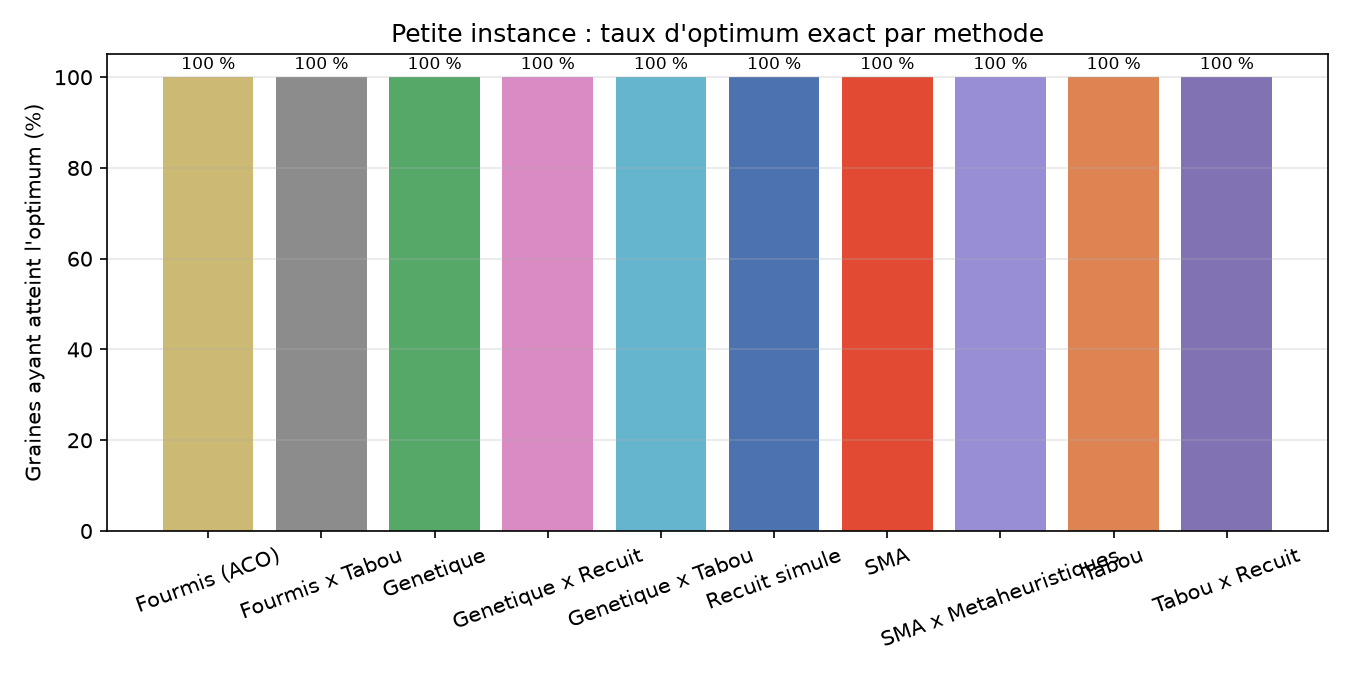
\includegraphics[width=0.95\linewidth,height=0.38\textheight,keepaspectratio]{petite_taux_optimum.png}
      \credit{10/10 méthodes à l'optimum exact.}
    \end{column}

    \begin{column}{0.50\textwidth}
      \centering
      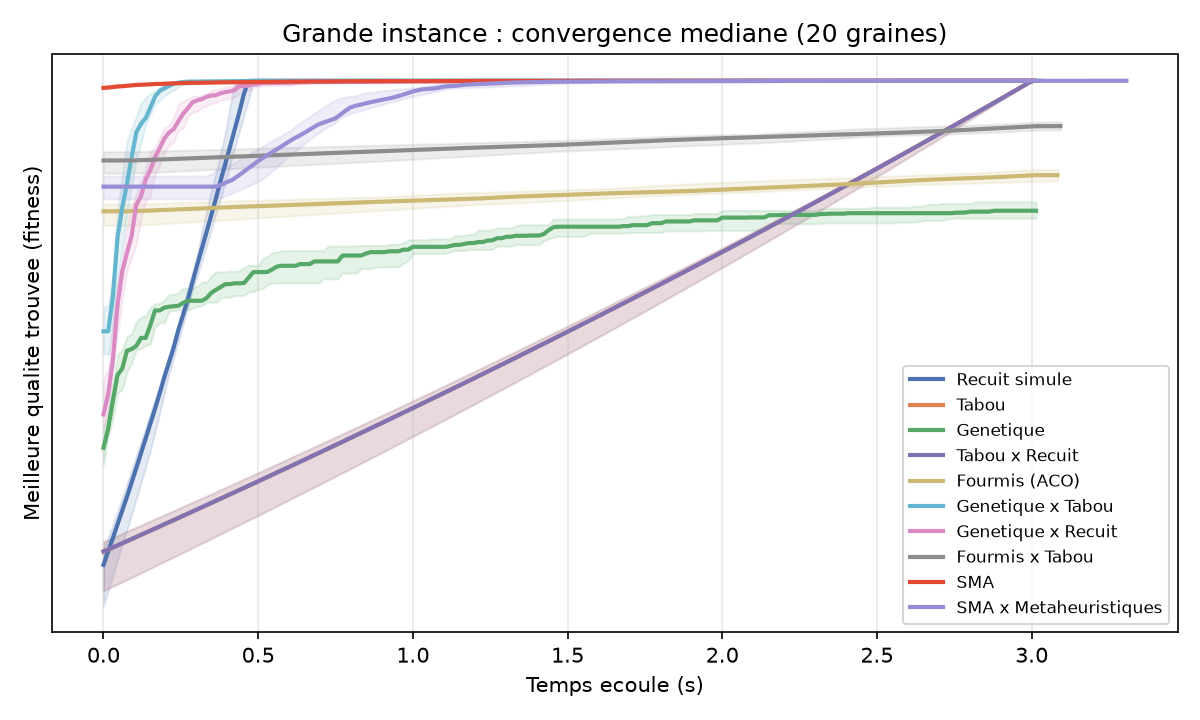
\includegraphics[width=\linewidth,height=0.44\textheight,keepaspectratio]{grande_convergence.png}
      \credit{Convergence médiane, 300 patients, 3 s, 20 graines.}
      \uncover<2->{\par\vspace{0.12cm}\footnotesize Le planning est optimal
        pour les durées prévues. Une urgence,\textbf{ une annulation ou une salle
        fermée suffit à le rendre inadapté.}}
    \end{column}
  \end{columns}
\end{frame}

\begin{frame}{Aléas : les quatre cas principaux}
  \scriptsize
  \begin{block}{Quatre aléas principaux}
    \begin{itemize}
      \item \textbf{Urgence} : patient imprévu, fenêtre temporelle imposée ;
        à insérer dans une vacation compatible.
      \item \textbf{Annulation} : patient programmé qui annule ; libère un
        créneau \textbf{et} des lits.
      \item \textbf{Indisponibilité de lits} : capacité réduite sur un
        intervalle ; réaffecter les séjours chevauchants.
      \item \textbf{Retard bloc} : prolongation ou incident sur une
        vacation ; capacité utile réduite.
    \end{itemize}
  \end{block}

  \par\vspace{0.04cm}
  {\footnotesize \textbf{HAS 2026} : environ 10\,\% des interventions
    programmées sont annulées, la plupart reprogrammées.}

  \uncover<2->{%
  \par\vspace{0.10cm}
  \begin{columns}[T,onlytextwidth]
    \begin{column}{0.46\textwidth}
      \begin{block}{Statique}
        \footnotesize Un plan nominal, optimisé pour les durées prévues.
        C'est la référence de départ.
      \end{block}
    \end{column}
    \begin{column}{0.52\textwidth}
      \begin{exampleblock}{Dynamique}
        \footnotesize Le plan est maintenu dans le temps : dates de repli
        proactives, puis replanification réactive.
      \end{exampleblock}
    \end{column}
  \end{columns}}
  \source{Chaque aléa a sa classe et son simulateur reproductible
    (\texttt{generer\_scenario\_aleas}).}
\end{frame}

\begin{frame}{Dynamique : préparer des dates de substitution}
  \scriptsize
  \begin{columns}[T,onlytextwidth]
    \begin{column}{0.46\textwidth}
      \begin{block}{Quatre profils de repli}
        \begin{itemize}
          \item \textbf{Nominal} : planning optimal à 100\,\% de la capacité.
          \item \textbf{Robuste avec marge} : 15\,\% de capacité laissée libre
            (bloc + lits) pour absorber un aléa sans déplacer les patients.
          \item \textbf{Sécurité lits} : lissage strict, sous-saturation
            volontaire.
          \item \textbf{Date B} : bonne qualité, différente du nominal.
        \end{itemize}
      \end{block}
    \end{column}

    \begin{column}{0.52\textwidth}
      \footnotesize Une Date A optimale, une Date B alternative, avec leurs
      raisons.

      \par\vspace{0.12cm}
      \renewcommand{\arraystretch}{1.25}
      \centering
      \begin{tabular}{@{}p{1.9cm}p{1.45cm}p{1.45cm}p{1.75cm}@{}}
        \toprule
        Patient & Date A & Date B & Arbitrage \\
        \midrule
        Mme D. & 12 mars & 26 mars & lits tendus \\
        M. K. & 14 mars & 21 mars & bloc saturé \\
        Mme R. & 15 mars & 18 mars & équipe \\
        \bottomrule
      \end{tabular}

      \uncover<2->{\par\vspace{0.12cm}Le chirurgien voit la date, l'occupation
        du bloc et des lits, et la raison de l'écart.}
    \end{column}
  \end{columns}
  \source{Extraction : \texttt{extraire\_options\_date\_a\_b}.}
\end{frame}

\begin{frame}{Dynamique / réactif : replanifier sans tout déplacer}
  \scriptsize
  \begin{columns}[T,onlytextwidth]
    \begin{column}{0.53\textwidth}
      \begin{block}{Trois garde-fous}
        \begin{itemize}
          \item \textbf{Gel du passé} : actes commencés ou programmés
            sanctuarisés.
          \item \textbf{Urgences} : insertion prioritaire dans la fenêtre
            clinique.
          \item \textbf{Moindre perturbation} : limiter déplacements et
            changements de jour.
        \end{itemize}
      \end{block}

      \uncover<2->{%
      \begin{alertblock}{Score d'adaptation}
        \[
          \begin{aligned}
            \text{Score} = \text{Fitness}
            &- w_p \cdot \text{déplacements}\\
            &- w_j \cdot \text{changements de jour}
          \end{aligned}
        \]
        Le planning reste proche de celui annoncé aux patients.
      \end{alertblock}}
    \end{column}

    \begin{column}{0.45\textwidth}
      \centering
      \begin{tikzpicture}[
        ag/.style={draw=McmSage,rounded corners=2pt,fill=McmSage!10,
                   minimum height=0.55cm,minimum width=1.55cm,align=center,
                   font=\tiny},
        bb/.style={draw=McmTerracotta,rounded corners=2pt,
                   fill=McmTerracotta!10,minimum height=1.95cm,
                   minimum width=1.85cm,align=center,font=\tiny,thick},
        co/.style={draw=McmAmber,rounded corners=2pt,fill=McmAmber!10,
                   minimum height=0.5cm,minimum width=1.85cm,align=center,
                   font=\tiny},
        f/.style={-{Latex[length=1.7mm]},thick,draw=McmTerracotta}]
        \node[ag] (a1) at (0,0) {Agent recuit};
        \node[ag] (a2) at (0,-0.85) {Agent tabou};
        \node[ag] (a3) at (0,-1.70) {Agent génétique};
        \node[bb] (bb) at (2.55,-0.85) {\textbf{Tableau noir}\\meilleure\\solution};
        \node[co] (co) at (2.55,0.55) {\textbf{Coordinateur}};
        \draw[f] (a1.east) -- (bb.west|-a1);
        \draw[f] (a2) -- (bb);
        \draw[f] (a3.east) -- (bb.west|-a3);
        \draw[f,draw=McmAmber] (co) -- (bb);
      \end{tikzpicture}
      \uncover<2->{\par\vspace{0.10cm}\footnotesize Agents par cycles
        courts, versionnement de la meilleure solution, migration si
        stagnation.}
    \end{column}
  \end{columns}
  \source{Implémentation Mesa 3.5 : agents simples et agents
    métaheuristiques coopérant par tableau noir.}
\end{frame}

\againframe<4>{recap}

\section{Analyser les résultats}

\begin{frame}{Classement à budget de temps égal}
  \scriptsize
  \begin{columns}[T,onlytextwidth]
    \begin{column}{0.50\textwidth}
      \renewcommand{\arraystretch}{1.12}
      \setlength{\tabcolsep}{3pt}
      \begin{tabular}{@{}lrr@{}}
        \toprule
        Méthode & Écart & Rang \\
        \midrule
        Recuit simulé & \textbf{0,015} & \textbf{1,25} \\
        Tabou $\times$ Recuit & \textbf{0,018} & 1,75 \\
        Tabou & 0,240 & 3,55 \\
        Génétique $\times$ Tabou & 0,261 & 3,75 \\
        SMA & 1,078 & 5,05 \\
        SMA $\times$ Méta & 1,196 & 6,15 \\
        Génétique $\times$ Recuit & 2,031 & 6,50 \\
        Fourmis $\times$ Tabou & 1\,006,0 & 8,00 \\
        Fourmis (ACO) & 2\,031,2 & 9,00 \\
        Génétique & 2\,836,2 & 10,00 \\
        \bottomrule
      \end{tabular}
    \end{column}

    \begin{column}{0.48\textwidth}
      \centering
      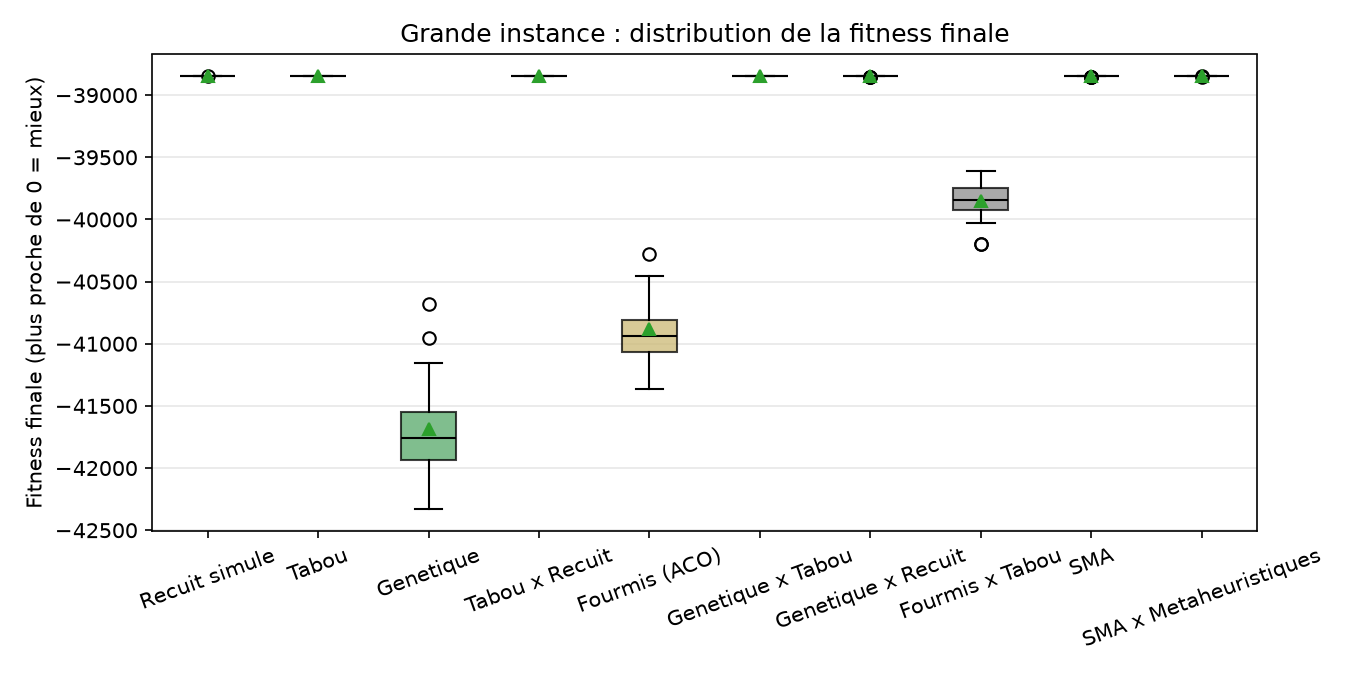
\includegraphics[width=\linewidth,height=0.30\textheight,keepaspectratio]{grande_boxplot.png}
      \credit{Dispersion de la fitness finale, grande échelle.}
      \uncover<2->{\par\vspace{0.12cm}\footnotesize Les méthodes locales
        dominent ; Génétique $\times$ Tabou et Fourmis $\times$ Tabou
        réduisent fortement l'écart. L'écart est mesuré à la meilleure
        solution observée.}
    \end{column}
  \end{columns}
  \source{Campagne \texttt{resultats/benchmark} : 300 patients, 80 vacations,
    20 graines, 3 s ; référence $-38\,847\,195$.}
\end{frame}

\begin{frame}{ML : durée, séjour, ambulatoire}
  \small
  \begin{columns}[T,onlytextwidth]
    \begin{column}{0.48\textwidth}
      \renewcommand{\arraystretch}{1.35}
      \centering
      \begin{tabular}{@{}lrrr@{}}
        \toprule
        Capacité & Médianes & Modèle & Oracle \\
        \midrule
        42 lits & 246 & \textbf{251} & 260 \\
        10 lits & \textbf{111} & 108 & 115 \\
        \bottomrule
      \end{tabular}
      \par\vspace{0.15cm}
      {\footnotesize
        MAE séjour : $1{,}11\rightarrow0{,}44$ jour\\
        F1 ambulatoire : \textbf{0,922}\\
        Intervalle à 90\,\% : $\pm1{,}02$ jour}
    \end{column}

    \begin{column}{0.50\textwidth}
      \footnotesize
      Le gain dépend des ressources.

      \uncover<2->{\par\vspace{0.12cm}À 42 lits, le modèle termine 5
        interventions de plus que les médianes, 9 de moins que l'oracle. À
        10 lits, la capacité sature : la prédiction ne crée pas de place.}
    \end{column}
  \end{columns}
  \source{Cas terminés sur 279, politique réactive, fermeture 10h--12h,
    2 salles, graine 0. Oracle = durées futures révélées, pas optimum
    garanti. Métriques ML : campagne interne de l'équipe.}
\end{frame}

\begin{frame}{SMA : ce que la coordination coûte}
  \small
  \begin{columns}[T,onlytextwidth]
    \begin{column}{0.48\textwidth}
      \renewcommand{\arraystretch}{1.30}
      \centering
      \begin{tabular}{@{}lrr@{}}
        \toprule
        Plan & Terminées / 279 & Dépass. (min) \\
        \midrule
        Figé & 255 & 2\,911 \\
        Réactif & 251 & \textbf{2\,716} \\
        \bottomrule
      \end{tabular}
    \end{column}

    \begin{column}{0.50\textwidth}
      \footnotesize
      Le compromis n'est pas systématique.

      \uncover<2->{\par\vspace{0.12cm}La replanification réduit le
        dépassement de 195 min, mais termine 4 interventions de moins.\par
        \vspace{0.08cm}Rang moyen : 5,05 à 300 patients, 5,85 à 582.\par
        \vspace{0.06cm}La solution reste versionnée et validée avant
        exécution.}
    \end{column}
  \end{columns}
  \source{279 interventions, 42 lits, 2 salles, salle 1 fermée 10h--12h,
    graine 0. Dépassement : occupation et remise en état après 17h.}
\end{frame}

\section{Montrer l'application}

\begin{frame}{KYST : le flux tiré jusqu'à la réservation}
  \small
  \begin{columns}[T,onlytextwidth]
    \begin{column}{0.58\textwidth}
      {\Large\bfseries\color{mcmPrimary} kyst.tech}\\[0.15cm]
      \textbf{Keep Your Surgeries Timely} : l'application web qui applique le
      flux tiré en consultation, du planning statique à l'adaptation dynamique.

      \vspace{0.12cm}
      \begin{exampleblock}{Trois gestes}
        \begin{itemize}
          \item saisir une demande en consultation ;
          \item obtenir deux dates, justifiées ;
          \item confirmer : vacation et lit sont réservés.
        \end{itemize}
      \end{exampleblock}

      \uncover<2->{\par\vspace{0.12cm}\footnotesize Planning statique initial,
        puis dynamique : dates de repli et replanification réactive. Disponible
        sur PC et mobile.}
    \end{column}

    \begin{column}{0.39\textwidth}
      \centering
      
\includegraphics[height=4.5cm]{qr_kyst.png}\\[0.25cm]
      {\footnotesize\bfseries Ouvrez KYST}\\[0.1cm]
      {\tiny Données synthétiques, aucune donnée réelle.}
    \end{column}
  \end{columns}
\end{frame}

\begin{frame}{Architecture : un socle standard, hébergé sur place}
  \scriptsize
  \centering
  \begin{tikzpicture}[
      card/.style={draw=McmTerracotta,rounded corners=2pt,fill=white,
                   minimum height=1.10cm,text width=1.85cm,align=center,
                   inner sep=3pt,font=\scriptsize},
      ext/.style={card,draw=McmMuted,dashed},
      flow/.style={{Latex[length=2mm]}-{Latex[length=2mm]},thick,draw=McmTerracotta},
      lab/.style={font=\tiny,text=McmMuted,inner sep=1pt}]
    \node[ext]  (user)  at (0,0)    {\textbf{Navigateur}\\PC ou mobile};
    \node[card] (front) at (3.2,0)  {\textbf{Front}\\SvelteKit};
    \node[card] (api)   at (6.4,0)  {\textbf{API}\\FastAPI};
    \node[card] (db)    at (9.6,0)  {\textbf{Base}\\PostgreSQL};
    \node[ext]  (ai)    at (6.4,-1.75) {\textbf{Modules IA}\\prédiction,\\ordonnanceur};
    \draw[flow] (user)  -- node[lab,above=2pt] {HTTPS} (front);
    \draw[flow] (front) -- node[lab,above=2pt] {interne} (api);
    \draw[flow] (api)   -- node[lab,above=2pt] {SQL} (db);
    \draw[flow] (api)   -- node[lab,right=2pt] {contrats Python} (ai);
    \begin{scope}[on background layer]
      \node[draw=McmSage,dashed,rounded corners=3pt,inner sep=4pt,
            fit=(front)(api)(db)(ai)] (srv) {};
    \end{scope}
    \node[font=\tiny,text=McmSage,anchor=south east] at ([shift={(0,1pt)}]srv.north east)
      {Podman rootless, Ansible};
  \end{tikzpicture}

  \vspace{0.12cm}
  \begin{columns}[T,onlytextwidth]
    \begin{column}{0.49\textwidth}
      \footnotesize Le navigateur ne parle qu'au front ; l'API garde les
      droits et les données.
    \end{column}
    \begin{column}{0.49\textwidth}
      \footnotesize Argon2, cookies HttpOnly/Secure, TLS, conteneurs
      rootless, données pseudonymisées.
    \end{column}
  \end{columns}
\end{frame}

\begin{frame}{Parcours 1/3 : le planning se construit}
  \small
  \centering
  \begin{tikzpicture}[
      c/.style={draw=McmTerracotta,rounded corners=3pt,fill=white,
                text width=2.55cm,minimum height=1.55cm,align=center,
                font=\scriptsize,inner sep=3pt},
      f/.style={-{Latex[length=2.2mm]},thick,draw=McmTerracotta}]
    \node[c] (a) at (0,0) {\textbf{1. Demande}\\patient, spécialité,\\durée estimée};
    \node[c] (b) at (3.25,0) {\textbf{2. Prédiction}\\salle, séjour,\\ambulatoire};
    \node[c] (c) at (6.50,0) {\textbf{3. Dates A/B}\\bloc, lits,\\raisons};
    \node[c] (d) at (9.75,0) {\textbf{4. Confirmation}\\vacation + lit\\réservés};
    \foreach \x/\y in {a/b,b/c,c/d} \draw[f] (\x) -- (\y);
  \end{tikzpicture}

  \par\vspace{0.25cm}\footnotesize Le calcul contraint entre dans le
  parcours clinique, pas dans un tableur séparé.
\end{frame}

\begin{frame}{Parcours 2/3 : le bloc bouge}
  \small
  \renewcommand{\arraystretch}{1.45}
  \setlength{\tabcolsep}{4pt}
  \begin{tabular}{@{}p{3.3cm}p{5.1cm}p{4.9cm}@{}}
    \toprule
    \textbf{Aléa} & \textbf{Ce que fait l'outil} & \textbf{Ce que voit l'équipe} \\
    \midrule
    Salle 1 fermée 10h--12h & replanifie les cas en attente ; les actes
      commencés finissent & le planning avant/après, les cas déplacés \\
    Patient à déplacer & cherche le meilleur créneau compatible & les
      autres patients bougent le moins possible \\
    Chirurgien absent & déplace les actes non commencés & les créneaux
      libérés sont réutilisables \\
    \bottomrule
  \end{tabular}

  \uncover<2->{\par\vspace{0.15cm}\footnotesize Le passé est gelé ; une
    proposition invalide est rejetée et l'ancien plan reste actif.}
\end{frame}

\begin{frame}{Parcours 3/3 : l'urgence arrive}
  \small
  \centering
  \begin{tikzpicture}[x=1.0cm,y=1cm,>=Latex]
    \draw[very thick,draw=McmInk] (0,0) -- (11.0,0);
    \draw[line width=7pt,draw=McmAmber] (3.8,0) -- (5.4,0);
    \foreach \x/\lab in {0/08h,2.2/10h,4.4/12h,7.0/14h,11.0/17h} {
      \draw[draw=McmInk] (\x,-0.12) -- (\x,0.12);
      \node[below=5pt,font=\scriptsize] at (\x,0) {\lab};
    }
    \node[above=16pt,text=McmAmber,font=\scriptsize\bfseries] at (4.6,0)
      {Urgence : fenêtre clinique};
    \draw[line width=3pt,draw=McmSage] (4.0,0.28) -- (5.2,0.28);
    \node[text=McmSage,font=\tiny,anchor=west] at (7.8,0.45)
      {vert : créneau retenu};
  \end{tikzpicture}

  \vspace{0.25cm}
  \begin{columns}[T,onlytextwidth]
    \begin{column}{0.49\textwidth}
      \begin{block}{Ce que fait l'outil}
        \begin{itemize}
          \item insère l'urgence dans sa fenêtre ;
          \item décale le minimum de patients futurs ;
          \item recalcule, valide, puis propose.
        \end{itemize}
      \end{block}
    \end{column}
    \begin{column}{0.49\textwidth}
      \uncover<2->{\footnotesize L'outil ne décide pas seul de décaler un
        patient : la proposition est soumise au praticien, avec son motif.}
    \end{column}
  \end{columns}
\end{frame}

\begin{frame}{Déploiement : sur le serveur de l'établissement}
  \footnotesize
  \begin{columns}[T,onlytextwidth]
    \begin{column}{0.48\textwidth}
      \begin{block}{Ce qui s'installe}
        \begin{itemize}
          \item application web : PC, tablette, téléphone ;
          \item SvelteKit, FastAPI, PostgreSQL ;
          \item conteneurs rootless, déploiement Ansible.
        \end{itemize}
      \end{block}
    \end{column}

    \begin{column}{0.50\textwidth}
      \footnotesize
      Tout reste chez l'établissement.

      \uncover<2->{\par\vspace{0.12cm}Hébergement de données de santé,
        journal d'audit, sauvegardes et droits par rôle.}
    \end{column}
  \end{columns}
  \source{Version actuelle ; ouverture : qualification CE et RGPD.}
\end{frame}

\begin{frame}{Conformité : CE, RGPD et non-substitution}
  \footnotesize
  \begin{columns}[T,onlytextwidth]
    \begin{column}{0.48\textwidth}
      \begin{block}{Marquage CE / MDR}
        \begin{itemize}
          \item Logiciel d'aide à la décision : qualification au titre du
            règlement (UE) 2017/745.
          \item Avant mise sur le marché : marquage CE, dossier technique,
            gestion des risques.
          \item Après mise sur le marché : matériovigilance et mise à jour.
        \end{itemize}
      \end{block}
    \end{column}

    \begin{column}{0.50\textwidth}
      \begin{alertblock}{RGPD et données de santé}
        \begin{itemize}
          \item Minimisation : uniquement les données nécessaires.
          \item Pseudonymisation, hébergement de données de santé (HDS),
            accès par rôle.
          \item Base légale, droits des personnes, journal d'audit.
        \end{itemize}
      \end{alertblock}
    \end{column}
  \end{columns}

  \vspace{0.12cm}
  \begin{columns}[T,onlytextwidth]
    \begin{column}{0.48\textwidth}
      \textbf{Couvert} : dates A/B, réservation, prédictions, replanification.
    \end{column}
    \begin{column}{0.50\textwidth}
      \textbf{À compléter} : audit exhaustif, lissage week-ends et vacances.
    \end{column}
  \end{columns}

  \uncover<2->{\par\vspace{0.18cm}\centering Le praticien confirme chaque
    programme ; la qualification CE et la conformité RGPD restent à instruire.}
  \source{Règlement (UE) 2017/745 ; RGPD (UE) 2016/679.}
\end{frame}


\begin{frame}{Références}
  \scriptsize
  \begin{itemize}
    \item HAS, \emph{Organisation en unité de chirurgie ambulatoire et IQSS},
      rapport d'analyse, avril 2026.
    \item HAS, \emph{La chirurgie ambulatoire en 12 questions}, avril 2012.
    \item Règlement (UE) 2017/745 relatif aux dispositifs médicaux.
    \item Règlement (UE) 2016/679 (RGPD).
    \item Amin, Baldacci, Kayvanfar, \emph{A comprehensive review of operating
      room planning and scheduling problems}, 2024.
    \item Rachuba, Reuter-Oppermann, Thielen, \emph{Integrated planning in
      hospitals: a review}, 2024.
    \item Lex et al., \emph{Using machine learning to predict-then-optimize
      elective surgery scheduling}, 2025.
    \item Salezze Vieira, Machado Silva, Chaves, \emph{Random-key algorithms
      for integrated operating room scheduling}, 2025.
  \end{itemize}
\end{frame}

{\setbeamercolor{normal text}{fg=mcmPrimaryFg,bg=mcmPrimary!70}
\begin{frame}[plain,noframenumbering]
  \begin{center}
    \Large
    Merci de votre attention\\[0.5em]
    Questions ?
  \end{center}
\end{frame}
}

\end{document}
